\graphicspath{{./figures}}

\section{PocketQube Unit}
A block diagram of the system components for the PocketQube unit is shown in Figure \ref{fig:pqunit_system}.

\begin{figure}[!htb]
  \centering
  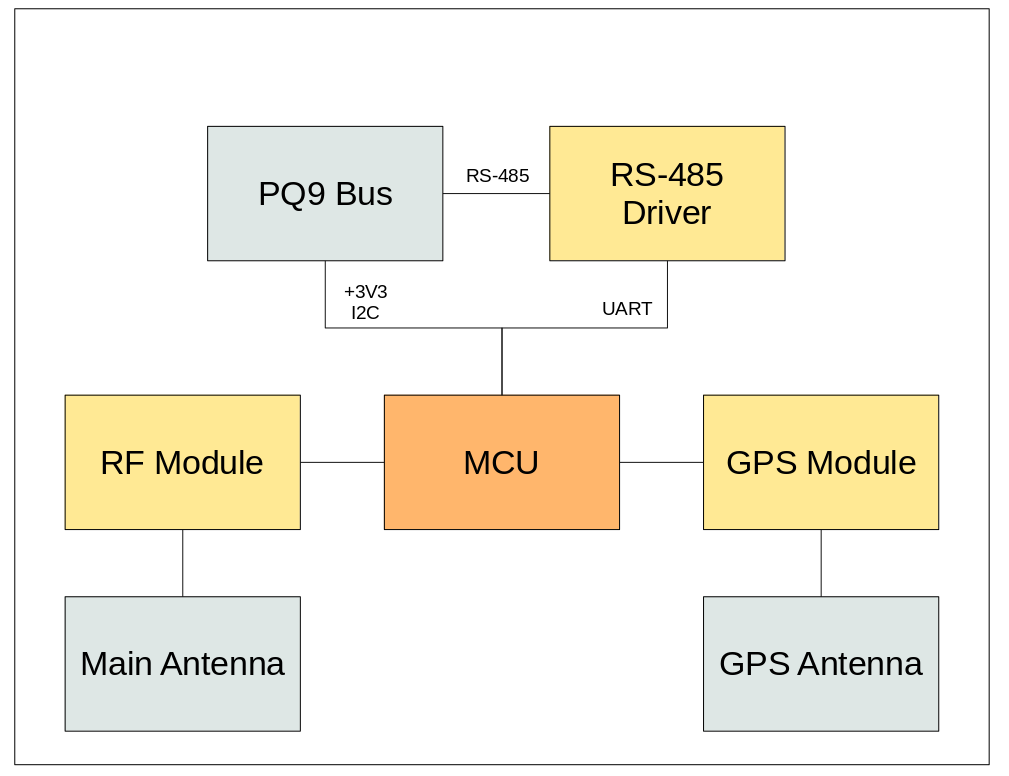
\includegraphics[width=0.6\textwidth]{pqunit_system}
  \caption{PocketQube Unit System Diagram}
  \label{fig:pqunit_system}
\end{figure}

This unit is relatively simple in comparison to the ground station, and so the ground station should be considered a priority. The unit consists of an RF section, and a GPS section. The RF antenna should integrate well onto a typical PocketQube housing, as should the GPS antenna. The MCU should be capable of interfacing with the Stellenbosch PocketQube bus, which includes:
\begin{itemize}
    \item A 3V3 line
    \item A 5V line
    \item An I2C bus
    \item An RS-485 bus
\end{itemize}
\noindent The MCU will pull directly from the +3V3 line, and will also communicate directly with the I2C bus. However, an RS-485 line transceiver should be included to cater for the RS-485 protocol, which will connect to the MCU via UART.